%% This is an example first chapter.  You should put chapter/appendix that you
%% write into a separate file, and add a line \include{yourfilename} to
%% main.tex, where `yourfilename.tex' is the name of the chapter/appendix file.
%% You can process specific files by typing their names in at the 
%% \files=
%% prompt when you run the file main.tex through LaTeX.

\chapter{Introduction}

\AddToShipoutPictureBG*{%
  \AtPageUpperLeft{%
    \hspace*{18.25cm}%
    \raisebox{-3cm}{%
      \makebox[0pt][r]{\parbox{\textwidth}{\begin{flushright}\textit{``It was the best of times, it was the worst of times.''}\\
      Charles Dickens\end{flushright}}}
}}}%

This research is motivated by the energy and environmental concerns we face in the context of increasing global climate change and massive urban growth. In general, it aims to potentially provide a step toward improving the urban sustainability.

\section{The need}

Global concern about depletion of non-renewable energy resources and anthropogenic climate change has become increasingly prevalent in recent years \cite{stocker2014climate}. Over the next decade, the United Nations predicts that we need to plan and build new homes for billions of city-dwellers worldwide \cite{united2015world}. \textit{Homo sapiens} has evolved into \textit{homo urbanus} \cite{grimond2007world}. This unprecedentedly continuous urbanization, if shaped merely by informal or inadequate policy measures, can potentially lead to worrisome consequences for the built environment, the economy at national or international level, and the well-being of humanity at large. 

In response to mitigating these on-going threats, the IPCC \cite{stocker2014climate} urges dramatic reduction in greenhouse gas (GHG) emissions and sustainable adaption of societies to a new climate context. Many governmental administrations have prioritized, among other actions, decarbonizing the energy system and reducing GHG emissions at local or global scales in order to achieve a clean-energy economy \cite{obama2017irreversible}. While the magnitude of GHG emissions varies among different cities, the building-related emission is always a key contributor. Urban systems need to be better understood to effectively tackle these problems in existing or new neighborhoods, not only which current sectors may cause the environmental issues but also what future changes may best reduce the energy consumption. Furthermore, in some cases the anthropogenic climate change can be exacerbated by neighborhood-to-city-scale phenomena, such as the heat islands.

As cities develop, the urban areas are gradually filled by tall buildings and canyons with dense blocks of structures, forming different morphologies relative to rural terrain. Besides, more urban surfaces exposed to the environment lead to higher effective albedo, increased effective thermal inertia, lower wind velocity, and decreased convective heat removal. Added to this is the anthropogenic heat gain due to human activities and the lower evaporation due to vegetation reduction. As a consequence, the outdoor air temperatures in cities tend to be different from those in rural areas, a phenomenon known as the Urban Heat Island (UHI) effect\footnote{Sometimes, the urban-rural temperature difference could be negative (especially in the morning), which is called the Urban Cool Island (UCI) effect.} \cite{oke1973city}.

The urban microclimate strongly depends on the urban surface layer. The latter is determined by the energy balance \cite{arnfield2003two, ooka2011thermal} between the received net radiation (both short-wave and long-wave), the sensible and latent heat fluxes transferred to the air, the heat storage in urban structures and the ground, and the anthropogenic heat sources, as shown in \textbf{Figure 1-1}. The energy-balance characteristics may vary \cite{salamanca2010new, grimmond1999heat} with city location, built form, urban geometry, surface materials, etc. So, the UHI effect tends to vary significantly from one location to another, and should be considered as site-specific.

\begin{figure}
\centering
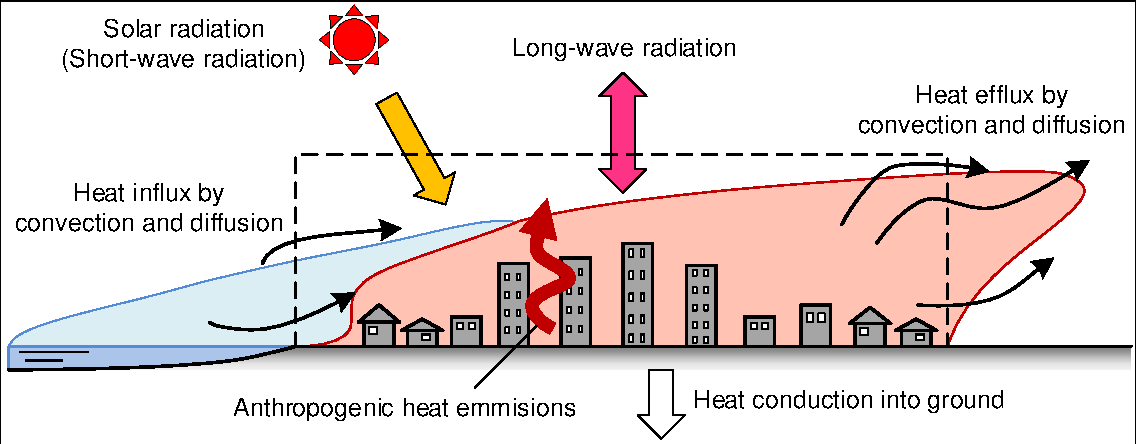
\includegraphics[width=.85\linewidth,trim=2 2 2 2.5,clip]{UHI.pdf}
\caption{Heat balance of the urban surface layer (mainly from Ref. \cite{ooka2011thermal}).}
\end{figure}

Regardless of the inherent uncertainties in predicting future climate and weather patterns, the UHI has been measured and documented throughout the world, including in Washington, DC, New York \cite{hicks2010heat}, Vancouver, Marseille \cite{lee2008vegetated}, London \cite{kolokotroni2012london}, Abu Dhabi \cite{martin2015estimation}, etc. In particular, Crawley \cite{crawley2008estimating} studied the UHI effect on an office building and suggested that the corresponding energy consumption could be modified between 5\% (increase in summer) and 10\% (decrease in winter). In order to meet the increasing peak demand in summer, more electricity generation by power plants will lead to higher emissions of VOCs, suspended particulates, and CO$_2$, as well as to aggravation of global warming and formation of harmful smog \cite{gorsevski1998air}. As a result, the UHI could indirectly cause various health problems leading to morbidity, disability, or even death \cite{gabriel2011urban}. Cities must undertake mitigation and adaptation measures to reduce the negative impacts of heat islands on the environment, the economy, and the population. However, aside from the social and economic concerns, developing effective adaptation strategies comes with a large technical challenge since an urban microclimate system comprises very complex physical relationships between many elements that may interact with each other \cite{masson2014adapting}. A good understanding of the mechanism and characteristics of UHI is thus a prerequisite for decision makers to identify and adopt reliable sustainability options, particularly during the design of new or renovated neighborhood areas.



\section{The state of the art}\label{ch1:opts}

\subsection{Urban-scale simulation model}
This pressing need motivates many energy and environment research communities to expand their scope to the urban realm \cite{reinhart2016urban}. Great efforts have been made to incorporate the UHI effect into thermal simulations \cite{salamanca2010new, crawley2008estimating, oxizidis2008computational}. In addition, some researchers have started to look at the physical behavior or causal factors of urban climate change and heat island effect via mesoscale computational fluid dynamics (CFD) simulations \cite{li2013multi}, analytical and empirical algorithms \cite{ignatius2015urban}, and physics-based urban canopy models \cite{lee2008vegetated}. As different models are developed for different uses, different spatial scales need to be clearly defined and different simulation models need to be elaborated in terms of their capabilities to predict corresponding energy and environmental conditions. Although the mesoscale models are regarded as state-of-the-art in atmospheric weather predictions \cite{roth2007review}, their applications still remain limited due to high computational cost and lack of boundary condition data.

As an alternative, Bueno et al. \cite{bueno2013urban} proposed and developed the Urban Weather Generator (UWG) to quickly estimate the UHI effect in the urban canopy layer and produce neighborhood-specific weather files, using the meteorological data measured at weather stations located in an open area outside the city. The UWG can also be considered as an offline bottom-up model to evaluate the building energy consumption at the neighborhood-to-city scale. It has been validated in Toulouse (France), Basel (Switzerland) \cite{bueno2013urban}, Singapore \cite{bueno2014computationally}, and Boston (USA) \cite{nakano2015urban}. With continuous improvements and updates \cite{yang2016curious}, the UWG has the potential to be a promising urban microclimate simulation engine that shows satisfactory performance with exceptionally low computational requirements.

However, despite the positive progress, simulation practice to date has only penetrated a small fraction of professional communities within the AEC industry. One recognized obstacle is the discrepancy, sometimes significant, between actual and predicted values. In general, prognostic law-driven models \cite{saltelli2008global} involve a suite of simplified physical relations describing the way various component disturbances (from system operation, human activity, material property, etc.) interact with each other and influence the aggregate physical behavior. Within these equations, both differential and algebraic, hundreds or even thousands of parameters exist. It is common for an engineer to make ad-hoc estimates for these parameters based on limited engineering knowledge, past user experience, and an abundance of trial and error. As a result, even though many inputs seem empirically validated, the simulated output could be far from the real scenario. It is ironic that at the time when simulation is the most popular, parameters of simulation may be the least reliable, which inevitably reduces the confidence of simulated results and curtails the use of simulation models to some extent. It is hence necessary to match simulation with measurement, a process called ``model calibration.''

\subsection{Model uncertainty and sensitivity}

Although some studies use calibrated models, their underlying calibration techniques are unclear. In order to dive deeper into model calibration, it is important to consider ``model uncertainty'' \cite{hopfe2011uncertainty}. Validation of a complex-system model is notoriously difficult, especially when the purpose of the model is to look at some non-observable or unmeasured physical behavior. The reason stems from the fact that closed-loop simulations usually represent major simplifications and constraints. That is to say, ``\textit{the portion of the world captured by the model is an arbitrary `enclosure' of an otherwise open, interconnected system}'' \cite{rosen1991life}. Model errors are mainly caused by difficulties in capturing how exactly a system operates, due to software limitations and inaccurate parameter descriptions that cannot be completely modeled a priori. The input parameters are often calibrated manually by an expert, which may require days or weeks of work depending on model complexity. A commonly observed method tunes some specific parameters until the result meets an acceptance criterion without any uncertainty analysis.

Uncertainty quantification is often time-consuming and requires additional efforts in the overall design and/or retrofit phase of an engineering system, but can provide more robust decisions. However, not all the modeled aspects have the same level of importance and not every input parameter offers the same contribution to error propagation. As a result, uncertainty analysis is usually coupled with sensitivity analysis to measure the relative importance of various input parameters \cite{tian2013review}. In general, a single simulation only evaluates one single point in the parameter space without taking uncertainties into account. Consequently, building designers or city planners often perform manual parametric simulations varying one factor at a time, which is referred to as local analysis. This is why some cynics would say that ``\textit{models can be made to conclude anything provided that suitable assumptions are fed into them}'' \cite{economist1998fallout}. As many inputs in the model are associated with some degree of uncertainty, due to changeable conditions or lack of knowledge about the exact value, sensitivity analysis of model parameters plays an important role in the simulation process in order to achieve valuable information and increase model confidence.

Sensitivity analysis (SA), presented by Saltelli et al. \cite{saltelli2004sensitivity}, is a measure of the effect of an input on the output. In general, given the input uncertainties, one is able to assess the uncertainty in the model response (uncertainty analysis), and eventually to identify the inputs that contribute most to that uncertainty (sensitivity analysis). Thus, SA can be of tremendous help in subsequent model analysis, including simulation-based optimization \cite{nguyen2014review}, meta-model analysis \cite{mao2016towards}, automatic model calibration \cite{heo2012calibration}, etc. The SA methods can generally be divided into local and global approaches \cite{saltelli2004sensitivity}. The local methods require fewer computations but are ill-suited for complex systems. The global methods are regarded as more versatile to handle non-linear, non-additive, and non-monotonic systems \cite{tian2013review}.

A brief literature review suggests that the global SA has been widely applied in building thermal simulations \cite{macdonald2002quantifying, heiselberg2009application, de2009identification, eisenhower2012uncertainty, nguyen2015performance, menberg2016sensitivity}. In addition, some researchers have started to look at the causal factors of urban microclimate and heat island via parametric studies \cite{salamanca2010new, lee2008vegetated, martin2015estimation, bueno2013urban, nakano2015urban, hamdi2008inclusion}. However, to the author's best knowledge, there is nearly no related work on performing the global SA in urban microclimate models with respect to a large multiplicity of factors. This is because the global SA approaches are so computationally expensive that most urban-scale simulations cannot afford them. Fortunately, with acceptable performances and exceptionally low computational requirements, the UWG could enable a first step toward the exploration of the global design space with various input parameters in urban simulations. Once the ``weak'' parameters are determined by SA, they could be set at nominal values, thereby reducing the parameter space and increasing the calibration efficiency. The remaining influential input set is considered by a more rigorous calibration process.

\subsection{Optimization-aided model calibration}

Given the evidence that manually tuning the parameters can be viewed as an optimization process, it is natural to think about using computers to implement calibration in automatic or semi-automatic means via optimization algorithms. Simulation-based optimization -- wherein a simulation model is embedded in the optimization -- has been increasingly applied in the building science community through mathematical and statistical methods to assist design analysis \cite{nguyen2014review, evins2013review, machairas2014algorithms} and model calibration \cite{reddy2006literature, coakley2014review, fabrizio2015methodologies}. A pioneering study was conducted by Wright \cite{wright1986optimised} in the 1980s, while the number of optimization-related papers has sharply increased since 2005 \cite{nguyen2014review}. Many open-source tools, such as the \textsc{GenOpt} by Wetter \cite{wetter2009generic}, are now available to provide the capabilities of coupling various building performance simulations to effectively support optimization.

Generally speaking, an objective performance function is formulated to define a max/min target, while some constraint functions are employed to reduce the possibility of deviating too far from the reality. Since the performance function asso-ciated with building or urban thermal-physical behavior is usually discontinuous, non-differentiable, multi-modal, and locally-flat \cite{wetter2004convergent}, traditional gradient-based algorithms cannot successfully search the whole parameter space. On the other hand, heuristic-based algorithms (e.g., evolutionary algorithm) have been frequently used in building or urban performance optimization, mainly owing to their abilities to obtain good solutions with some degree of efficiency and robustness. In particular, a brief literature review indicates that heuristic-based algorithms can perform reliable calibration for building energy models \cite{robertson2015reduced, yang2016automated, ruiz2016genetic, ruiz2017analysis}. To the author's best knowledge, there is nearly no work on performing optimization-based calibration of physics-based urban microclimate models, due partly to the expensive computational costs.

At the current stage, calibration still relies to some extent on expert judgment and engineering experience (e.g., in the selection of candidate inputs). So, we recognize that the computer is more likely to act as a supplement to optimize and accelerate the calibration by transforming manual adjustment into automatic tuning. However, application of numerical optimization in the calibration process, while abstracting the physical objective as a tractable mathematical problem, inevitably neglects some real physical details in the constraint(s). Indiscriminant use could result in mathematical match but physical mismatch, which is why some researchers would criticize such methodology. This naturally necessitates the incorporation of uncertainty analysis after calibration to test reliability.

Finally, although simulation-based optimization has been actively discussed, one practical concern is the computation time. A typical model optimization could take days or weeks of computation to find optimal or near-optimal solutions. Given the time-constrained nature of engineering applications, it is necessary to develop novel optimization methods that are able to find high-quality solutions as quickly as possible.

\section{The goal}

This study was initiated with the intention to account for uncertainty in developing more coherent and integrated strategies concerning the energy and environmental issues in the urban system. The overall goal of this thesis is to identify a general methodology to the topic of automatic model calibration and apply it to an urban microclimate system. Essentially, the proposed ideas involve various concepts and methods borrowed from allied scientific disciplines in a more mathematical and statistical point of view. Corresponding analysis builds upon the newest Urban Weather Generator (UWG) to present a deep look into an existing district area located in downtown Abu Dhabi (UAE).

The core of the thesis is divided into \textit{two} parts, which correspond to two journal publications \cite{mao2017global,mao2018optimization} that have come out of this research. The first part is devoted to global sensitivity analysis, which is used to determine the relative impacts of input parameters on estimates of the urban outdoor air temperature. The second part is devoted to optimization-aided model calibration, which is used to auto-tune the selected input parameters so that the UWG model can represent the urban microclimate as precisely as possible. To the author's best knowledge, this is to date the first time to perform global sensitivity analysis and automatic calibration on physics-based urban microclimate models.

\textbf{Chapter 1} overviews the state of the art in urban microclimate simulation research and states the thesis goal. \textbf{Chapter 2} introduces the basic mechanism and major updates of the newest UWG for urban microclimate simulation. \textbf{Chapter 3} illustrates a baseline model of the selected case study for the proposed methodologies detailed in \textbf{Chapter 4}. In particular, we have developed a global regression-based sensitivity analysis, a Monte Carlo filtering technique, and an online hyper-heuristic evolutionary algorithm for the current research. Finally, results and discussions are provided in \textbf{Chapter 5}, and the corresponding conclusions and prospects for future work are outlined in \textbf{Chapter 6}.

The final achievement of this study is expected to be helpful in using simulation-based analysis as a deeper basis for providing the tool, guideline, recommendation, best-practice example, and background information to practitioners and researchers in the field of building and/or urban system study. In this sense, a modeling approach that is able to robustly integrate field measurements and computer simulations has the potential to significantly improve the way buildings and/or cities are designed and operated. This research aims to represent an initial step toward such promising vision.
